\chapter{Ecoulements visqueux}
\label{ch:newtonien}

\section{Equation de Navier-Stokes pour fluide Newtonien, incompressible}

Dans le chapitre~\ref{ch:euler}, nous avons établi l'équation d'Euler pour un fluide parfait, en négligeant les effets de la viscosité. Cependant, dans la réalité, les fluides réels (comme l'eau ou l'air) présentent une résistance interne au mouvement, due aux frottements entre couches de fluide. 


\begin{figure}
  \begin{center}
    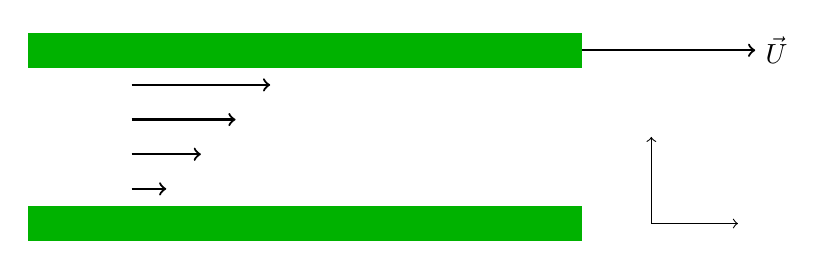
\begin{tikzpicture}[scale=2.2] % adjust scale so total width ≈ 6 cm
  \tikzset{plate/.style={fill=green!70!black, draw=none}}
  
  % Lower plate: from (-0.6,-0.1) to (2.6,0.1)
  \draw[plate] (-0.6,-0.1) rectangle (2.6,0.1);
  
  % Upper plate: from (-0.6,0.9) to (2.6,1.1)
  \draw[plate] (-0.6,0.9) rectangle (2.6,1.1);

  % Flow arrows at y = 0.2,0.4,0.6,0.8
  \draw[->, thick] (0,0.2) -- (0.2,0.2);
  \draw[->, thick] (0,0.4) -- (0.4,0.4);
  \draw[->, thick] (0,0.6) -- (0.6,0.6);
  \draw[->, thick] (0,0.8) -- (0.8,0.8);

  \draw[->] (3.,0) -- (3.5,0) node[right] {$\ex$};
  \draw[->] (3.,0) -- (3.0,0.5) node[above] {$\ez$};
  % Velocity arrow on the right side of the upper plate
  % Length approx = 1.0
  \draw[->, thick] (2.6,1.0) -- ++(1.0,0) node[right] {$\vec{U}$};
\end{tikzpicture}


  \end{center}
  \caption{Expérience idéalisée représentant la viscosité d'un fluide entre deux plaques présentant entre elles un différentiel de vitesse  $U$ sur une épaisseur $h$. La force par unité de surface ($A$) à exercer sur la plaque supérieure en régime stationnaire est $\od{\vec{F}}{A}= \mu U/h$}\label{fig:couette}
\end{figure}

On aborde la notion de viscosité dans le régime laminaire par l'expérience de l'écoulement de Couette. Soit une couche de fluide prise entre deux plaques présentant entre elles une différence de vitesse $\vec{U}$. Si le fluide est suffisament visqueux, la couche suffisament fine, et la vitesse suffisament petite (ce sont des éléments que nous allons préciser), la vitesse du fluide adopte un profil linéaire, sans glissement par rapport aux deux parois mobiles, et la force par unité d'aire ($A$) à exercer sur la plaque supérieure pour conserver un régime stationnaire  est $\od{\vec{F}}{A}=\mu \vec{U}/h$, ce qui est équivalent à affirmer que la force par unité d'aire exercée par le fluide sur cette plaque est $-\od{\vec{F}}{A}$. 

Cette force par unité de surface porte le nom de contrainte, et il s'agit plus particulièrement ici d'une \cindex{contrainte tangentielle}, notée $\tau_{xz}$:


\begin{displaymath}
  \tau_{xz} = \mu U/h
\end{displaymath}

Le premier indice, $x$, fait référence à la direction de la force (par unité de surface). L'indice $z$ fait référence s'exerce sur la face supérieure du fluide, dont la nomale est dirigée dans la direction de l'aexe $\ez$. Nous verrons dans peu de temps que $\tau_{xz}$ est la composante d'un \cindex{tenseur des contraintes}. 

\todo{dans le schéma, utiliser la notation $\tau$}

L'expérience est idéalisée à beaucoup d'égards et il ne faut pas se laisser distraire par les intéractions spécifiques entre le fluide et la plaque. Le point important est que le fluide présente une \emph{résistance au cisaillement}. Nous pouvons formaliser le phénomène à l'échelle d'un élement fluide. Considérons trois éléments, empilé selon l'axe $\ez$, caractérisés par une vitesse horizontale $U(z)$. A l'échelle de ce volume élémentaire, l'expression linéaire adoptée pour l'écoulement de Couette suggère que le bloc supérieur exerce une force de composante horizontale  $\dif F_x = -\mu \od{U}{z}(z+\frac{1}{2}\dif z)\dif x\dif y$ sur le bloc intermédiaire, et le bloc inférieur exerce une force de composante horizontale $\dif F_x = \mu \od{U}{z}(z-\frac{1}{2}\dif z)\dif x\dif y$. 

On peut donc modéliser la somme des forces de viscosité, par unité de volume, dans cet écoulement laminaire $U(z)$ par 

\begin{equation}
  \dif F_x = \od{}{z} \mu \od{U}{z} \dif V =  \mu \od[2]{U}{z} \dif V. 
  \label{eq:newtonnien}
\end{equation}

On est donc tenté de compléter le raisonnement qui a a abouti à l'équatieur d'Euler \eqref{eq:euler} pour y intégrer ce phénomène de viscosité. Considérons d'abord exclusivement l'effet d'un cisaillement selon $\ez$, sur la composante $\ex$ de la vitesse:

\begin{displaymath}
  \rho \, \Dt{u_x} = - \rho \, \grad \gpot - \grad p + \mu \od[2]{u_x}{z} 
\end{displaymath}

Par symmétrie, un cisaillement selon $\ey$ aura le même effet, qui doit donc être ajouté à la même équation

\begin{displaymath}
  \rho \, \Dt{u_x} = - \rho \, \grad \gpot - \grad p + \mu ( \od[2]{u_x}{x} + \od[2]{u_x}{y} )
\end{displaymath}

Avec un peu d'audace, nous pourrions suggérer qu'un différentiel de vitessse selon l'axe $\ex$ génère une force que l'on peut paramétriser de la même manière (résistance à l'étirement):

\begin{equation}
  \rho \, \Dt{u_x} = - \rho \, \grad \gpot - \grad p + \mu ( \od[2]{u_x}{x} + \od[2]{u_x}{y} +  \od[2]{u_x}{z} )
  \label{eq:diffusion_ux}
\end{equation}

On peut justifier notre audace en reconnaissant, dans l'équation \eqref{eq:diffusion_ux} un analogue à l'équation de la chaleur. De la même façon que l'énergie se diffuse par l'effet cumulé des chocs moléculaires, la quantité de mouvement de \emph{diffuse}, également par échange lors des collisions. L'analogie est très imparfaite car en réalité les force d'attractions jouent un rôle majeur dans le phénomène de diffusion. Nous allons donc admettre cette équation. Elle est bien correcte. C'est l'équation de Navier-Stokes pour un fluide newtonien incompressible, mais elle doit être justifiée plus soigneusement. C'est l'objet de la section \ref{sect:ns}. 

\begin{figure}
  \begin{center}
    \begin{tikzpicture}[scale=1.0]

% Styles
\tikzset{
  outer/.style={dotted, draw=black, line width=0.4pt},
  middle/.style={draw=black, line width=1.5pt},
  force/.style={->, thick, blue!70!black},
  vel/.style={->, line width=1pt},
}

% --- Three rectangles ---
% Left block
\draw[outer] (-1,-1) rectangle (2,0);

% Middle block (thick)
\draw[middle] (-0.8,0) rectangle (2.2,1);

% Right block
\draw[outer] (-0.6,1) rectangle (2.4,2);

% --- Axes arrows ---
\draw[->, thick] (-3.2,0) -- (-3.2,1.0) node[midway,left] {$\ez$};
\draw[->, thick] (-3.2,0) -- (-2.2,0) node[midway,below] {$\ex$};

% --- Velocity vectors on middle block ---
% Coordinates of centers of top and bottom faces of middle block
\coordinate (bottomcenter) at (0.7,-0.1);
\coordinate (topcenter)    at (0.7,1.1);
\coordinate (bottomright) at (2.3,0);
\coordinate (topright)    at (2.3,1.0);

% Velocities (black)
\draw[vel] (bottomright) -- ++(0.8,0)
  node[right] {$U\!\left(z-\tfrac12 \,\mathrm dz\right)$};

\draw[vel] (topright) -- ++(1.0,0)
  node[right] {$U\!\left(z+\tfrac12 \,\mathrm dz\right)$};

% Force vectors (dark green)
\draw[force] (bottomcenter) -- ++(0.5,0.0)
node[below] {$\mu\,\frac{\mathrm dU}{\mathrm dz}\!\left(z-\frac{1}{2} \dif z \right)$};

\draw[force] (topcenter) -- ++(-0.5,+0.0)
node[above] {$\mu\,\frac{\mathrm dU}{\mathrm dz}\!\left(z+\frac{1}{2} \dif z\right)$};

% Dots at centers
\fill (bottomright) circle (1.5pt);
\fill (topright) circle (1.5pt);

% --- Dimension markers ---
% Height = dz
\draw[<->] (-1.2,0. ) -- (-1.2,1. )
  node[midway,left] {$\dif z$};

% Length = dx
\draw[<->] (-1.0,-1.3) -- (2.0,-1.3)
  node[midway,below] {$\dif x$};

\end{tikzpicture}




  \end{center}
  \caption{Bilan des forces de viscosité causées par le cisaillement sur un volume élémentaire}
\end{figure}


En trois dimensions, cette équation de Navier-Stokes devient: 

\begin{displaymath}
  \rho \Dt{\u} = -\grad p - \rho \grad \gpot + \mu \lapl \u,
\end{displaymath}
où $\lapl \u = (\lapl u_x, \lapl u_y, \lapl u_z)$ est le \cindex{laplacien} du champ de vitesse, et $\mu$ le \cindex{coefficient de viscosité}. 

Quelques valeurs typiques pour différents fluides à température ambiante :

\begin{center}
\begin{tabular}{|c|c|c|}
\hline
Fluide & $\mu$ (Pa$\cdot$s) & Conditions \\
\hline
Eau & $10^{-3}$ & 20$^\circ$C \\
\hline
Air & $1.8 \times 10^{-5}$ & 20$^\circ$C, 1 atm \\
\hline
Huile moteur & $0.1$ & 20$^\circ$C \\
\hline
Miel & $10$ & 20$^\circ$C \\
\hline
\end{tabular}
\end{center}
Cette équation sera suffisante pour décrire la plupart des écoulements étudiés dans ce cours, y compris l'\cindex{écoulement de Poiseuille}.





\section{Tenseur des contraintes}

Dans le chapitre~\ref{ch:euler}, nous avons utilisé la \cindex{pression statique} pour décrire les forces normales s'exerçant sur un élément de volume de fluide. Nous avions écrit explicitement :
\begin{displaymath}
  \dif\vec{f} = p \vec{n} \dif A.
\end{displaymath}
Cette expression suppose que la force est purement normale à la surface, ce qui est valable pour un fluide parfait.
Or, nous l'avons vu, la viscosité se manifeste par des forces \emph{tengentielles} à la surface témoin. Ces forces sont proportionnelles à la surface témoin (comme les forces de pressions) mais il nous faut un formalisme mathématique qui permette d'exprimer leur caractère directionnel. C'est l'objet du \cindex{tenseur des contraintes}, $\tensor{\tau}$. La force associée à ce tenseur est maintenant directionnelle (contrairement à sa forme dans \eqref{eq:hydrostat_int} et \eqref{eq:hydrostat_diff}:


\begin{displaymath}
  \dif\vec{f} = \tensor{\tau} \vec{n} \dif A.
\end{displaymath}

Ce tenseur permet de prendre en compte non seulement les forces normales (pression), mais aussi les forces tangentielles (cisaillement). 

On retrouve le fluide parfait pour  $T_{ij} = -p \delta_{ij}$, soit $\tensor{T} = -p \tensor{\delta}$.

\todo{donner un exemple deux 2 des contraintes dans une dimension . ou alors laisser ça au modèle de Stokes}

L'enjeu est de développer une expression de $\tau$ pour le fluide Newtonien. C'est l'objet de la section suivante. 

\begin{redmargin}
  \section{Dérivation formelle de l'équation de Navier-Stokes \label{sect:ns}}

Pour paramétrer $\tensor{\tau}$, nous partons du \cindex{tenseur des déformations} $\tensor{e}$, défini comme la partie symétrique du gradient de vitesse :
\begin{displaymath}
  e_{ij} = \frac{1}{2}\left( \pd{u_i}{x_j} + \pd{u_j}{x_i} \right).
\end{displaymath}
Ce tenseur capture les effets de compression, dilatation et cisaillement du fluide. En supposant que le fluide est newtonien (c'est-à-dire que les contraintes sont proportionnelles aux déformations) et isotrope (les propriétés sont indépendantes de la direction), on montre que le tenseur des contraintes visqueuses s'écrit :
\begin{displaymath}
  \tau_{ij} = 2 \mu e_{ij} + \lambda \delta_{ij} \sum_{m} e_{mm},
\end{displaymath}
où $\mu$ est le coefficient de viscosité dynamique et $\lambda$ le second coefficient de viscosité. La somme $\sum_{m} e_{mm}$ n'est autre que la divergence du champ de vitesse, $\Div \u$.

En combinant ce résultat avec la pression statique, on obtient le tenseur des contraintes total :
\begin{equation}
  T_{ij} = - \left( p + \frac{2}{3} \mu \Div \u \right) \delta_{ij} + 2\mu e_{ij}.
  \label{eq:stress_tensor}
\end{equation}
La trace de ce tenseur, $\sum_i T_{ii}$, donne accès à la pression dynamique $\bar{p}$ :
\begin{displaymath}
  \bar{p} = -\frac{1}{3} \text{Tr}(\tensor{T}) = p + \left( \frac{2}{3}\mu + \lambda \right) \Div \u.
\end{displaymath}
La partie déviatorique du tenseur (de trace nulle) est associée au cisaillement :
\begin{displaymath}
  T_{ij} = - \bar{p} \delta_{ij} + \left( 2 \mu e_{ij} - \frac{2}{3}\mu \Div \u \delta_{ij} \right).
\end{displaymath}
L'\cindex{approximation de Stokes} suppose que $p = \bar{p}$, ce qui implique $\lambda = -\frac{2}{3}\mu$. Dans ce cas, le tenseur des contraintes se simplifie en :
\begin{equation}
  T_{ij} = - p \delta_{ij} + 2\mu e_{ij} - \frac{2}{3}\mu \Div \u \delta_{ij}.
  \label{eq:tenseur_contraintes_stokes}
\end{equation}
Pour un fluide incompressible ($\Div \u = 0$), cette expression se réduit à :
\begin{equation}
  \tensor{T} = - p \tensor{\delta} + 2 \mu \tensor{e}.
  \label{eq:tenseur_contraintes_stokes_incompressible}
\end{equation}


En insérant cette expression dans l'équation du mouvement, on remplace la force de pression par la divergence du tenseur des contraintes :
\begin{equation}
  \rho \, \Dt{\vec{u}} = - \rho \, \grad \gpot - \Div{\tensor{T}}.
  \label{eq:ns}
\end{equation}
La divergence du tenseur $\tensor{T}$ est définie par composante par composante. La composante $i$ répond à
\begin{displaymath}
  (\Div{\tensor{T}})_i = \sum_j \pd{T_{ij}}{x_j}.
\end{displaymath}
En développant ce terme pour un fluide incompressible et en utilisant l'approximation de Stokes, on retrouve (après un peu de calcul) l'équation de Navier-Stokes incompressible :
\begin{equation}
  \rho \Dt{\u} = -\grad p - \rho \grad \gpot + \mu \lapl \u.
  \label{eq:ns_incompressible}
\end{equation}
Cette équation décrit la dynamique des fluides visqueux et sera la base de nos prochains développements, notamment pour l'étude des écoulements laminaires comme celui de Poiseuille.
\end{redmargin}

\section{Écoulements de Poiseuille}

\subsection{Écoulement de Poiseuille plan ($\pd{p}{x} = C$, $u_x(0) = u_x(h) = 0$)}

\todo{remettre contexte}

Si le gradient de pression est constant ($\pd{p}{x} = C$) et que les deux plaques sont fixes, les conditions aux limites imposent $B = 0$ et $A = 0$. Le profil de vitesse est alors parabolique :
\begin{displaymath}
u_x(y) = \frac{C}{2\mu} (y^2 - h y).
\end{displaymath}

Le débit volumique par unité de largeur est :
\begin{displaymath}
Q = \int_0^h u_x(y) \, \dif y = -\frac{C h^3}{12\mu}.
\end{displaymath}

\subsection{Écoulement de Poiseuille dans un cylindre}
\label{sec:poiseuille_cylindre}

En coordonnées cylindriques, l'équation de Navier-Stokes pour un écoulement stationnaire ($\pd{}{t}=0$), axisymétrique ($p=p(r)$; $u_x=u_x(r)$, $u_r=0$)) et incompressible se réduit à :
\begin{displaymath}
0 = -\od{p}{x} + \frac{\mu}{r} \od{}{r}\left( r \od{u_x}{r}\right).
\end{displaymath}

On peut retrouver cette équation en exprimant les opérateurs différentiels en coordonnées cylindriques, mais nous pouvons également la retrouver en raisonnant sur un bilan de forces. 

Considérons, le long de l'écoulement,  un anneau de fluide de rayon $r$ et d'épaisseur $\dif r$ (figure~\ref{fig:anneau_cylindre}).

\begin{figure}[h]
  \begin{minipage}[b]{0.55\textwidth}
\input{Pdftex/05_cylindre_couette.pdf_tex}
\end{minipage}\hfill
\begin{minipage}[b]{0.4\textwidth}
\caption{Schéma d'un anneau de fluide dans un cylindre. Les forces de pression et de cisaillement sont indiquées.}
\label{fig:anneau_cylindre}
\end{minipage}
\end{figure}

Les forces agissant sur cet anneau sont :
\begin{itemize}
    \item Force de pression : $-2\pi r \od{p}{x} \dif r$.
    \item Force visqueuse : La contrainte de cisaillement $\tau_{rx} = \mu \od{u_x}{r}$ agit sur les surfaces interne et externe de l'anneau. La force nette est
    \begin{displaymath}
    2\pi \dif x \left( \tau_{rx}(r+\dif r)(r + \dif r) - \tau_{rx}(r) r \right) = 2\pi \dif x  \od{}{r}\left( r \mu \od{u_x}{r}\right) \dif r.
    \end{displaymath}
\end{itemize}

L'écriture  $\tau_{rx}(r+\dif r)(r + \dif r)$ est ambiguë: elle exprime $\tau_{rx}$ évaluée en $r + \dif r$, multipliée par la longueur $r + \dif r$. 

L'équilibre des forces donne:
\begin{displaymath}
0 = -2\pi r \od{p}{x} + 2\pi \mu \od{}{r}\left( r \od{u_x}{r}\right), 
\end{displaymath}

ce qui est bien notre équation. Nous pouvons maintenant la résoudre. 

La solution de cette équation, avec la condition aux limites $u_x(a) = 0$, est :
\begin{displaymath}
u_x(r) = \frac{a^2 - r^2}{4\mu} \od{p}{x}.
\end{displaymath}

Le débit volumique $Q$ est obtenu en intégrant sur la section du cylindre :
\begin{displaymath}
Q = \int_0^a u_x(r) 2\pi r \, \dif r = -\frac{\pi a^4}{8\mu} \od{p}{x}.
\end{displaymath}

\subsection{Validité de l'approximation}

ICI: c'est le moment d'attirer l'attention sur les conditions relatives à la symmétrie, et l'absence de termes d'advection. Nous avons donc considérer que la symmétrie du problème se reflète dans la symmétrie des lignes de courant, ce qui génère $\pd{u}{x}=0$ et $\pd{u}{r}=0$  donc annihile tous les termes d'advection. En pratique c'est ce qu'on appelle un écoulement laminaire et developpé. 

 \begin{itemize}
     \item Le nombre de Reynolds est faible ($Re \ll 1$) (ATTENTION: PAS ENCORE DEFINI).
     \item Le tuyau est suffisamment long pour que les effets d'entrée soient négligeables.
 \end{itemize}
%
TODO: Une analyse des ordres de grandeur permet de déterminer à quelle distance de l'entrée du tuyau ces hypothèses sont satisfaites.


% \section{Ecoulement dans un plan}
%
% but: développer une intuiton. 
%
% D'abord montrer sur un element de volume. Bien montrer comment le $\pd[2]{u}{x}$ apparaît (c'est la différence de stress entre haut et bas, et le stress lui même est fonction de la dérivée). 
%
% Ecoulement stationnaire, dans le plan (x,y), $u_x$ est constant, dont pas de terme d'advection. On écrit l'équation pour $u_x$ en faisant l'hypothèse $u_x=u_x(y)$. Il vient que l'équation se réduit à  (on ne tient pas compte du gradient de géopotentiel)
%
% TODO: faire une figure
%
% \begin{align*}
%   0 = -\pd{p}{x} + \od[2]{u}{y}
%   0 = -\pd{p}{y} 
% \end{align*}
%
% La solution est donc $p$ constant selon y, et en intrégrant deux fois la première équation on a: 
%
% \begin{displaymath}
%   A y + B = -\frac{y^2}{2} \od{p}{x} + \mu u
% \end{displaymath}
%
% Montrer plusieurs cas de figure: $\pd{p}{x}=0$ mais différence de vitesse (écoulement de couette), ensuite $\pd{p}{x}=C$ mais vitesse nulle aux bords (profile parabolique - écoulement de Poiseuille plan). 
%
%
% \section{Ecoulement de Poiseuille dans un cylindre}
%
% Ensuite attaquer le flux dans un cylindre. Dire qu'il y a deux approches. On prend brutalement l'expression de l'équation de la vitesse en coordonnées cylindriques : ça va tout seul. Ou bien on prend le temps de voir que la différence de pression sur un anneau doit compenser la différence de stress entre l'extérieur de l'anneau et l'intérieur. Les deux raisonnements aboutissent à la même équaiton
%
% \begin{displaymath}
%   0 = -\od{p}{x} + \frac{\mu}{r} \od{}{r}\left( r \od{u}{r}\right)
% \end{displaymath}
%
% avec la solution
%
% \begin{displaymath}
%   u(r) = \frac{r^2-a^2}{4\mu}\od{p}{x}
% \end{displaymath}
%
%
% On calcule le débit 
% \begin{displaymath}
%   \int_{0}^{a}u(r) 2\pi\, r\,\dif r=-\frac{\pi a^4}{8\mu}\od{p}{x}
% \end{displaymath}
%
% si pertinent on peut ensuite se demander 'à quelle profondeur du tuyau' tout cela est acceptable. Cela introduit une première analyse des ordres de grandeur. 

\section{Ecoulement très visqueux outour d'une sphère}

Formule de stokes \cite[][sect. 7. p.223]{acheson01aa}

Implication pour la sédimentation
